\section{APPLICATIONS}

If the \BCNs\ we research is online observable, and we have built the directed graph for them, then we can use the online observability to determine the initial states of these {\em BCNs}. Using the the online observability, it will need less observation costs to determine the initial state of this {\em BCN}. Furthermore we can also use it to try to find the shortest path or avoid entering critical states when we determine the initial state of {\em BCNs}. %Because the output we observe is not sure, we use expected value and variance of the length of path and the times of entering critical states to help us to choose the input.

\subsection{Determine the Initial State}

After we build the directed graph of the {\em BCN}, we can use it to determine the initial state of \BCNs\ as {\em Fig.\ref{fig:5}} shows. 
\begin{itemize}
  \item Firstly, we observe the output of the {\em BCN} mentioned before. If we observe the output is $\delta_4^1$ then we can infer that the possible states set should be $\{\delta_{16}^1,\delta_{16}^2,\delta_{16}^3\}$, and we record them as initial states and current states in the table. 
  \item After that we input  $\delta_4^1$ and observe the output is $\delta_4^3$ then we can infer that the possible states set should be $\{\delta_{16}^{10},\delta_{16}^{11}\}$, and we record them as current states set in the corresponding position. 
 \item Repeat the second step untill the cardinal number of the possible states set turns into $1$. In that time we can determine the current state and the corresponding initial state of the {\em BCN}.
\end{itemize} 
%Input and output again and again 

\begin{figure}[thpb]
      \centering
      \framebox{\parbox{3in}{
		\centerline{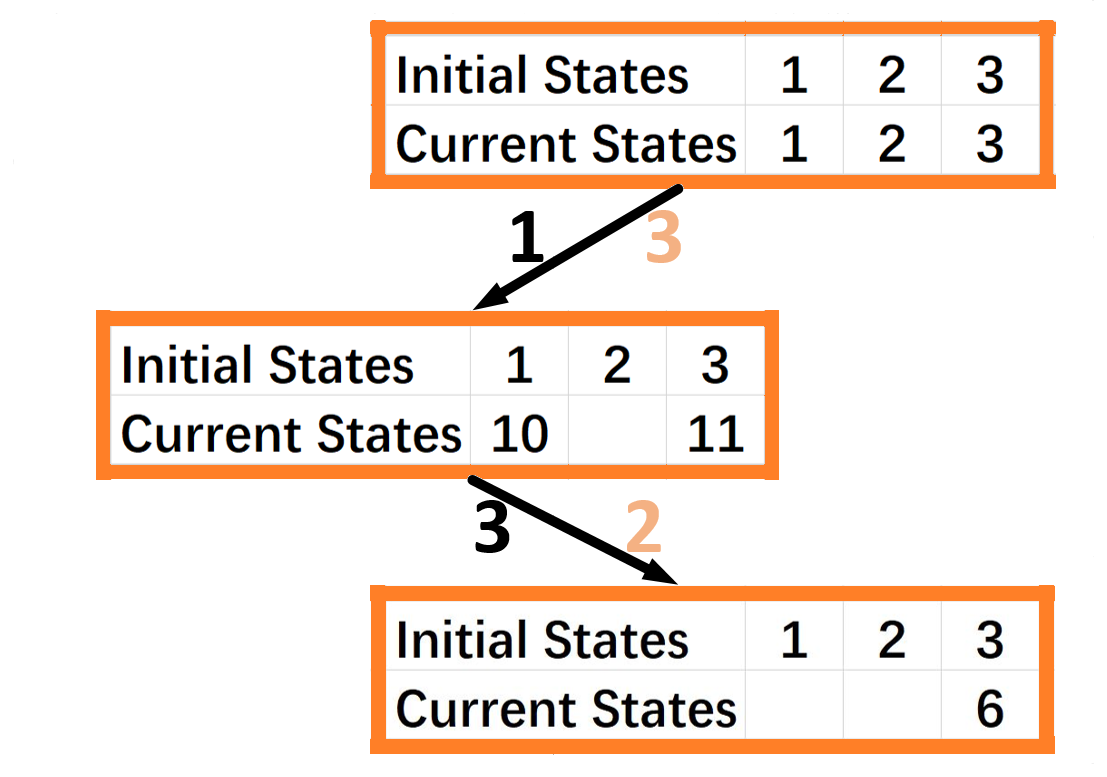
\includegraphics[scale=0.266]{figures/Fig5.png}}
	}}
      
      \caption{The process of determing the initial state of BCNs, we change the values of current states by input and the output we observe. }
      \label{fig:5}
   \end{figure}
\subsection{Less Observation Costs}
Some biological systems, such as the immune systems which can be depicted as the \BCN\ T-cell receptor kinetics model \cite{Klamt2006A}. There exist $3$ input-nodes, and $37$ state-nodes in this model, therefore the model has $2^3$ inputs and $2^{37}$ states. For the purpose of obtain the initial state of the {\em BCN}, we must select some state-nodes to be observe at first. 

If we use the online observability of \BCNs\ to determine the initial state of the \BCN\ T-cell receptor kinetics model, it needs less observation costs. Because compare with the existing third and fourth kind of observabilities the online observability need weakest preconditions to determine the initial state of {\ BCNs} without any presupposition. In other words, the {\ BCNs} needs less output-nodes to determine its initial state. As we can select less state-nodes to be observe, it will takes less ovservation costs in this example. In addition to this, there are also some other advantages, when we use the online observability of {\em BCNs}.

\subsection{Find Shortest Path}
When we need to determine the initial state of a {\em BCN}, an important aspect that we will consider is to find the shortest path. In general, we can't find the shortest path definitely.  Fortunately, we can use the directed graph to make the best decision. For the path, we introduce two functions {\tt Pe}$(S, I_z)$ and {\tt Pv}$(S, I_z)$ to describe its expected value and variance, respectively. For better explain our idea, we list some definitions in the following.
%We introduce two functions $Spe(S_i, I_i)$ and $Spv(S_i, I_i)$ to describe the expected value of the shortest path and variance of shortest path , $S_i$ is the possible states set and $I_i$ is the input we chose, the definition of $Spe(S_i, I_i)$ is as follows:\\
%With the $Spe(S_i, I_i)$ and $Spv(S_i, I_i)$ we can make the decision we like.


Some statements before definitions:
\begin{itemize}
  \item $\{I_1,I_2,\ldots, I_p\}$ : the right inputs set of $S$;
  \item $\{S_z^1,S_z^2,\ldots, S_z^k\}$ : the set of state sets, and its elements corresponding to the possible outputs $\{O_1,O_2,\ldots,O_k\}$ after input $I_z$, for every $I_z$ in $\{I_1,I_2,\ldots, I_p\}$.
 % \item the fourth one implies the third one, second one and first one.
\end{itemize} 
\begin{definition}[{\tt Spe}$(S)$] \label{lspe}
 \[{\tt Spe}(S)= \min({\tt Pe}(S, I_1),{\tt Pe}(S, I_2),\ldots,{\tt Pe}(S, I_p)).\] 
\end{definition}

\begin{definition}[{\tt Pe}$(S, I_z)$] 
When the $|S|=1$, we have that
{\tt Pe}$(S, I_z)=0$  for every $I$ in $\Delta_M$. According {\em Definition \ref{lspe}}, {\tt Spe}$(S)=0$ if $|S|=1$. But when the $|S|>1$, 
%and the $\{I_1,I_2,\cdots, I_p\}$ is the right inputs set of $S_i$. For every $I_i$ in $\{I_1,I_2,\cdots, I_p\}$ the $\{S_i^1,S_i^2,\cdots, S_i^k\}$ is a set of state sets whose elements corresponding to the possible outputs after input $I_i$, then 
we have that  
\[{\tt Pe}(S, I_z)=1 +\frac{\sum_{j=1}^k Spe(S_z^j)|S_z^j|}{ |S|}\] 
%and 
%\[{\tt Spe}(S_i)= \min({\tt Pe}(S_i, I_1),{\tt Pe}(S_i, I_2),\cdots,{\tt Pe}(S_i, I_p))\]
\end{definition}

The function shortest path  expected value {\tt Spe}$(S)$ is to find the $I_z$ from $\{I_1,I_2,\cdots, I_p\}$ to calculat least {\tt Pe}$(S, I_z)$ for $S$. From the definition of {\tt Pe}$(S, I_z)$ we can know that if $|S|=1$ then we can make sure the state of {\em BCNs}, and we need not input anymore to determine the state of {\em BCNs}. Therefore, for any input the path expected value {\tt Pe}$(S, I_z)$ would be $0$ and so do the shortest path  expected value {\tt Spe}$(S_i)$. But if $|S|>1$ we still need more input and observe the output. Only by this way we can determine the state of of {\em BCNs}. Therefore,  we can recursively define the {\tt Pe}$(S, I_z)$ and {\tt Spe}$(S)$ for each input $I_z$ in the right inputs set.  The {\tt Pv}$(S, I_z)$ can be defined in the similar way. Hence we omit the details in this paper. 

\subsection{Avoid Entering Critical States}
In biological systems, some states of the genes may corresponding to unfavorable or dangerous situations \cite{Li2014Controllability}. So another important aspect that we will consider is to avoid entering critical states. We can also construct two functions {\tt Ce}$(S, I_z)$ and {\tt Cv}$(S, I_z)$ to describe expected value and variance of the times of entering critical states, the definition of {\tt Ce}$(S, I_z)$ is as follows:\\
\begin{definition}[{\tt Lce}$(S)$] \label{lce}
\[{\tt Lce}(S)= \min({\tt Ce}(S, I_1),{\tt Ce}(S, I_2),\ldots,){\tt Ce}(S, I_p)\]
\end{definition}
\begin{definition}[{\tt Ce}$(S, I_z)$] 
When the $|S|=1$, and for every $I_z$ in $\Delta_M$, we have: \[{\tt Ce}(S, I_z)=|S \cap S_{cri} |\] 
According {\em Definition \ref{lce}}, %{\tt Spe}$(S_i)=0$ if $|S_i|=1$ 
\[{\tt Lce}(S)={\tt Ce}(S, I_z)=|S \cap S_{cri} |\] 
But when the $|S|>1$ 
%and the $\{I_1,I_2,\cdots, I_p\}$ is the right inputs set of $S_i$. For every $ I_i$ in $\{I_1,I_2,\cdots, I_p\}$ the $\{S_i^1,S_i^2,\cdots, S_i^k\}$ is a set of state sets whose elements corresponding to the possible outputs after input $I_i$, then 
we have that 
\[{\tt Ce}(S, I_z)=|S \cap S_{cri} | +\frac{\sum_{j=1}^k {\tt Lce}(S_z^j)|S_z^j|}{ |S_z|} \] 
%and 
%\[{\tt Lce}(S_i)= \min({\tt Ce}(S_i, I_1),{\tt Ce}(S_i, I_2),\cdots,){\tt Ce}(S_i, I_p)\]
\end{definition}

Where $S_{cri}$ is the critical states set of the {\em BCN} we research. The definition of {\tt Ce}$(S, I_z)$ has some difference with {\tt Pe}$(S, I_z)$, because we need to use the critical states set $S_{cri}$. So that  we can analyze the possibility of entering the  critical states when we infer the possible states set of {\em BCNs}.

We can get the definitions of {\tt Cv}$(S, I_z)$ in similar ways, and use all of these four functions to make the best decision we like. When we choose an input $I_z$ with least {\tt Pe}$(S, I_z)$, we may find the shortes path to determine the initial state. But the output of \BCNs\ after input $I_i$ is uncertain, so selecting the least $Pe(S, I_z)$ may leads to a very long path to determine the initial state of {\em BCNs}. For better performce, we the can also use the {\tt Pv}$(S, I_z)$ to avoiding risks. The uses of {\tt Ce}$(S, I_z)$ and {\tt Cv}$(S, I_z)$ are similar to {\tt Pe}$(S, I_z)$ and {\tt Pv}$(S, I_z)$, when we trying to avoid entering critical states of {\em BCNs}.

In the four existing kinds of observability, we can not analyze the state of \BCNs\ dynamically, so it would be hard to find the best way we like when we determine the initial state of {\em BCNs}. But this problem can be solved by the online observability of {\em BCNs}.